\chapter{Method}

\section{Choice of Method}


\begin{figure}[h]
%\hspace*{-0.4cm}
\begin{center}
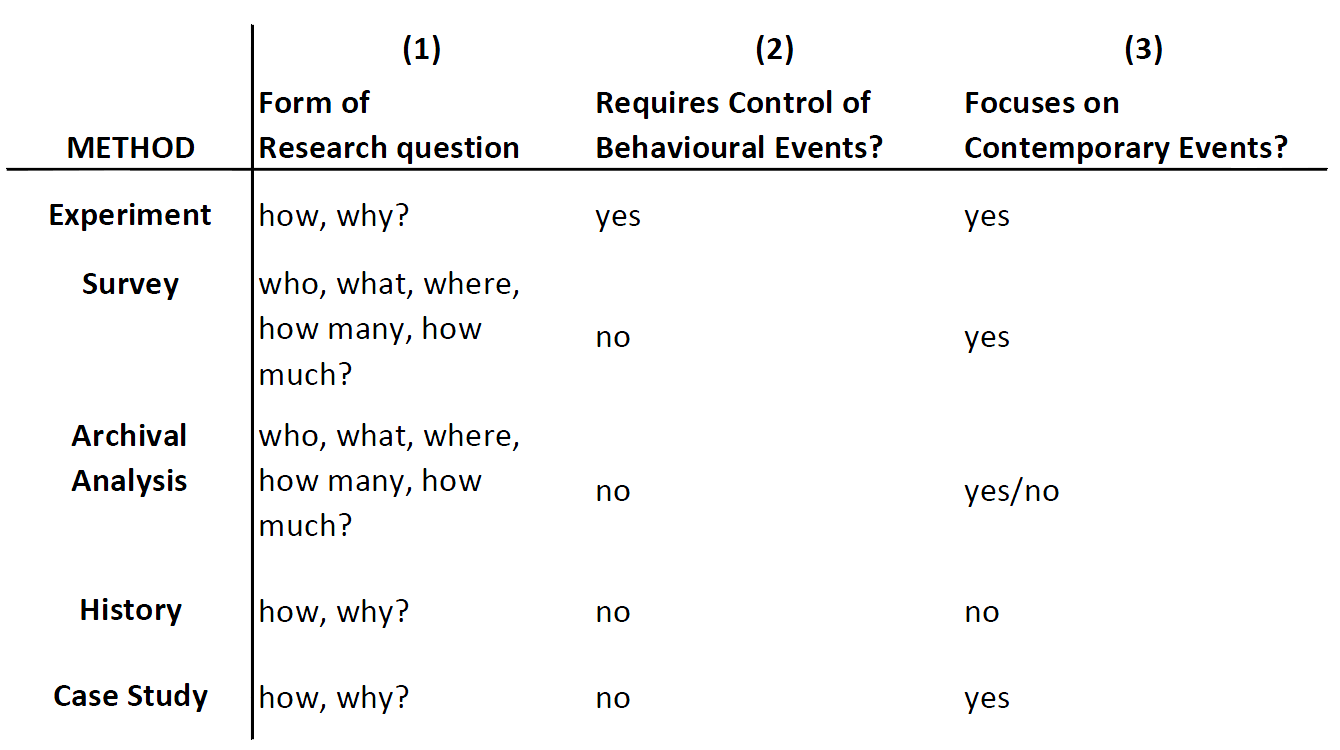
\includegraphics[scale=0.35]{methods.png}
\caption[Situations for different research methods]{Situations for different research methods, derived from \cite{CaseStudyResearch}}
\label{fig:methods}
\end{center}
\end{figure}

For the interviews in our study we chose a qualitative approach. This allowed us to focus on fewer and more in-depth interviews than with a quantitative approach, but eliminated the possibility to generalize the results. We chose to do semi-structured interviews conducted face-to-face. 

\section{Case Study}

%\cite{CaseStudyResearch}
%\cite{kitchenham1995case}
\subsection{Background Study}
\subsection{Semi-structured Interviews}
\subsection{Document study}
%\subsection{Action Research}

\section{Ethical Considerations}
%Litt i forhold til at man behandler sensitiv information og sånn
\subsection{Anonymization}

\section{Challenges}